%!TEX root = ../template.tex
%%%%%%%%%%%%%%%%%%%%%%%%%%%%%%%%%%%%%%%%%%%%%%%%%%%%%%%%%%%%%%%%%%%%
%% chapter3_HardwareDesign.tex
%% NOVA thesis document file
%%
%% Chapter with the Hardware Design part
%%%%%%%%%%%%%%%%%%%%%%%%%%%%%%%%%%%%%%%%%%%%%%%%%%%%%%%%%%%%%%%%%%%%

\typeout{NT FILE chapter3_HardwareDesign.tex}

\chapter{Hardware Design}\label{cha:chapter3_HardwareDesign}

Meter aqui um pequena introdução do que e mostrado neste capitulo e descrição de seccoes

\section{Architecture}\label{31_Architecture}

The system's desired specifications and requirements exposed throughout Section~\ref{sec:II_Specs} allow a redesign of its current architecture (Figure~\ref{fig:architecture_original}), which is presented in Figure~\ref{fig:architecture_new}.

% meter aqui o NOVO diagrama de blocos -- INACABADO;
\begin{figure}[h]
	\centering
	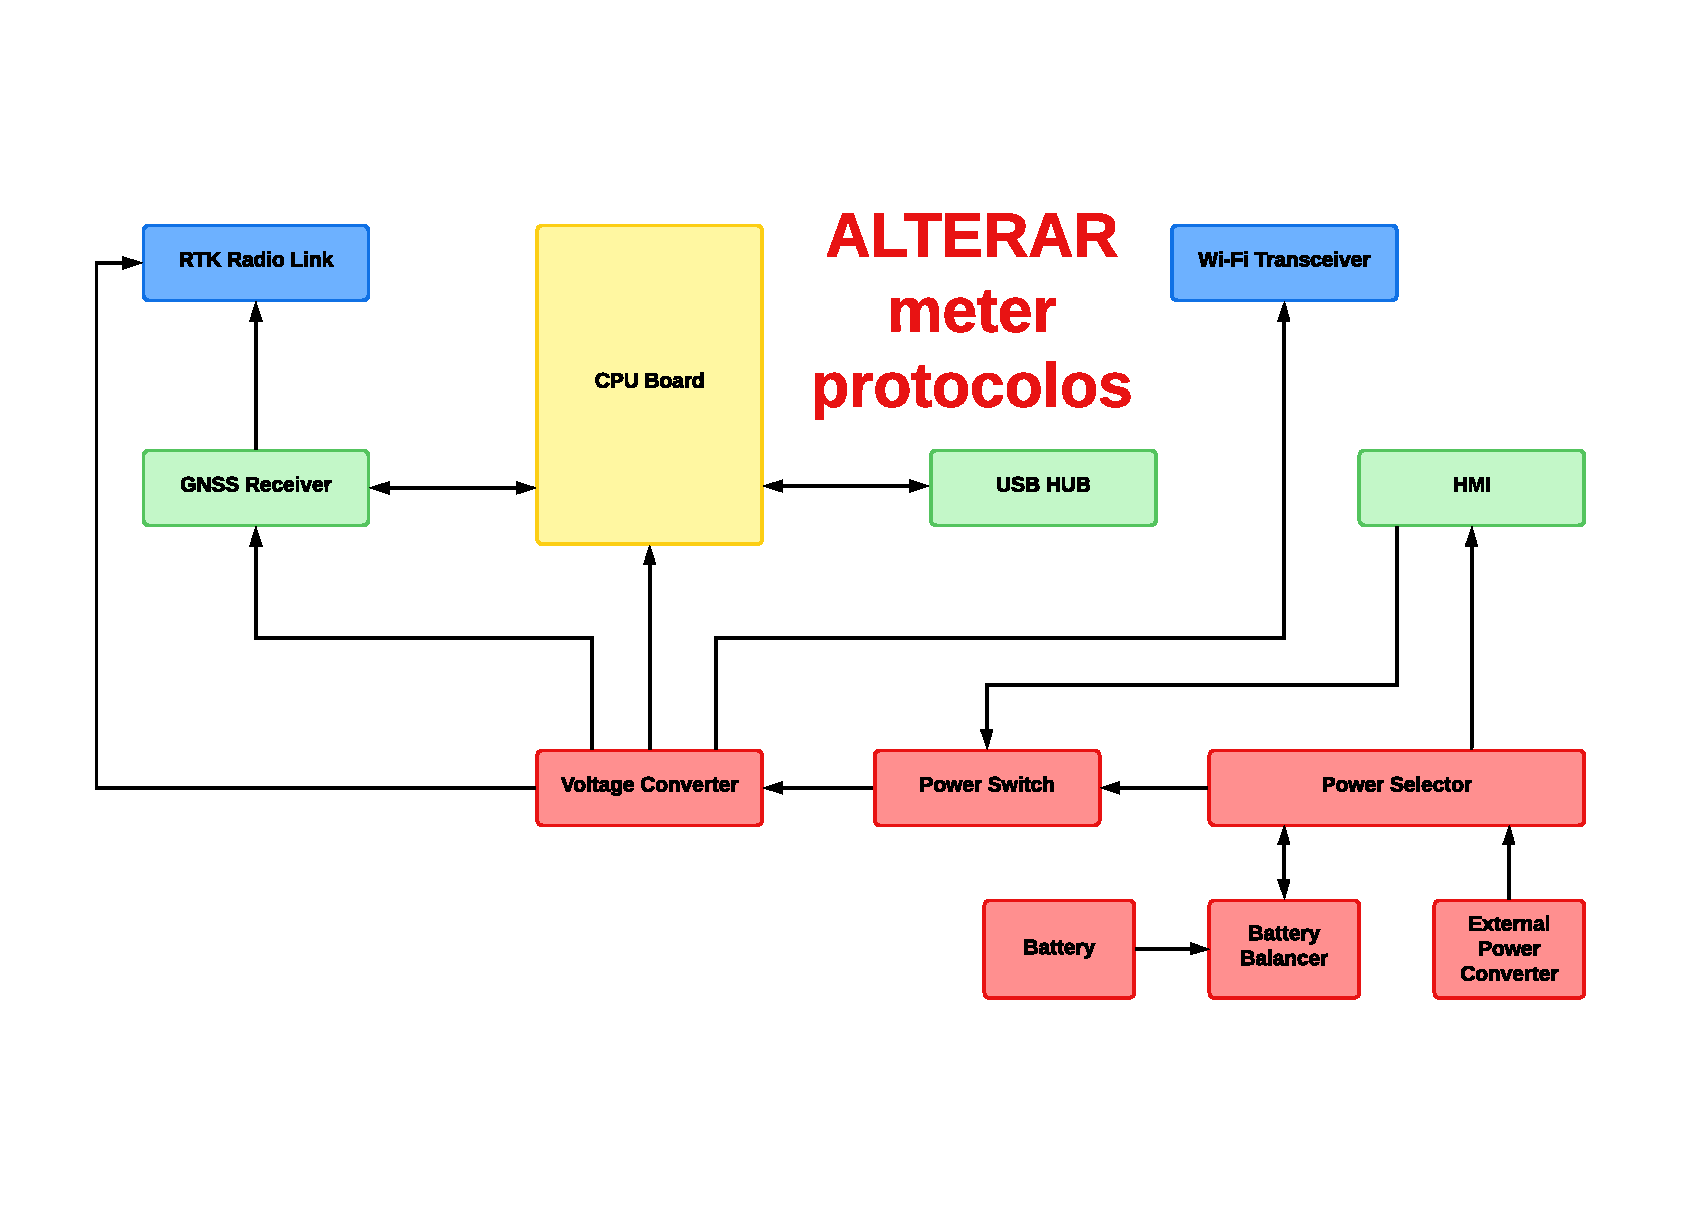
\includegraphics[width=1.0\textwidth]{Chapters/Figures/new_architecture.pdf}
	\caption{beRTK\textsuperscript{\textregistered} Base Station's redesigned block diagram.}
	\label{fig:architecture_new}
\end{figure}

Starting from the control subgroup, the only component to be selected was (ideally) a single-board computer able to replace the previously used Raspberry Pi 4 Model B. This means that the chosen device would have to be able to carry out a pre-determined set of instructions crucial for the operation of the base station. Such requirement is presented in Section~\ref{sec:II_FCT_requirements} -- requirement \textbf{RTKBS.MAIN.FCT.030}, which proposes the use of a single-board computer (SBC). The set of instructions performed by the original beRTK\textsuperscript{\textregistered} base station is carried out by a Raspberry Pi 4 Model B computer (described in Section~\ref{sec:II_architecture_Control}), therefore, an element with a comparable computational power as this computer would be ideal. The Raspberry Pi Foundation offers a variety of solutions for many project ideas, and since the operations intended for the beRTK\textsuperscript{\textregistered} base station are so well performed by the Raspberry Pi 4 Model B, it would be worth looking through the array of Raspberry Pi products in order to find a good solution. Research leads to the Raspberry Pi Compute Module 4. This compact module not only has a small form factor when compared with the Raspberry Pi 4 Model B, but it also bears its computational power thanks to the same processor (a Broadcom BCM2711 quad-core Cortex-A72 (ARM v8) 64-bit SoC @ 1.5GHz), which makes it a great option for the system's control unit.




The secondary power arrangement in the original beRTK\textsuperscript{\textregistered} design featured two external batteries that would feed the entire system once the mains power supply was disconnected. This form of supply poses considerable disadvantages when it comes to a continuous operation, due to the impractical need of removing the batteries in order to charge them. In the system's power supply subgroup, this was the main improvement to be made following the requirements defined in Section~\ref{sec:II_PWS_requirements}. For that, the base station's enclosure sould count on an internal battery that must not be removed (such battery could be comprised of either a single or multi-cell arrangement) on which the system could rely on once the external power supply was disconnected. This idea would help meet requirement \textbf{RTKBS.MAIN.MEC.030}, while also proposing a new issue, namely, the charging of the internal battery arrangement.
%meter LINK PARA CADA REQUIREMENT

The original beRTK\textsuperscript{\textregistered}'s design featured a prioritized PowerPath\textsuperscript{\texttrademark} controller, as mentioned in Section~\ref{sec:II_architecture_PowerSupply}. As per Analog Devices, a PowerPath\textsuperscript{\texttrademark} controller is a device able to control the flow of power through a system, while also selecting the power source itself.

Keeping in mind that the same GNSS receiver and Wi-Fi transceiver are going to be used in the new version of the base station, 

An ideal approach would be to find an IC able to 

With all this in mind, a wise starting point for the research of a power selector able to provide a smooth transistion between an external and internal supply would be from Analog Devices' power management ICs; specifically, from the battery charger ICs. The most well-suited IC found was LTC4012, which is a high efficiency, multi-chemistry battery charger with PowerPath\textsuperscript{\texttrademark} control~\cite{LTC4012}. This battery charger is able to

\section{Component Selection}\label{32_ComponentSelection}

\section{Circuit Design}\label{33_Circuit}

\section{PCB Layout Design}\label{34_PCBlayout}

